\documentclass[a4paper, 12pt]{article}
\usepackage{tikz}
\usepackage[margin=0.5cm]{geometry}

% a4paper size: 21cm x 29.7cm

\begin{document}
\pagestyle{empty}
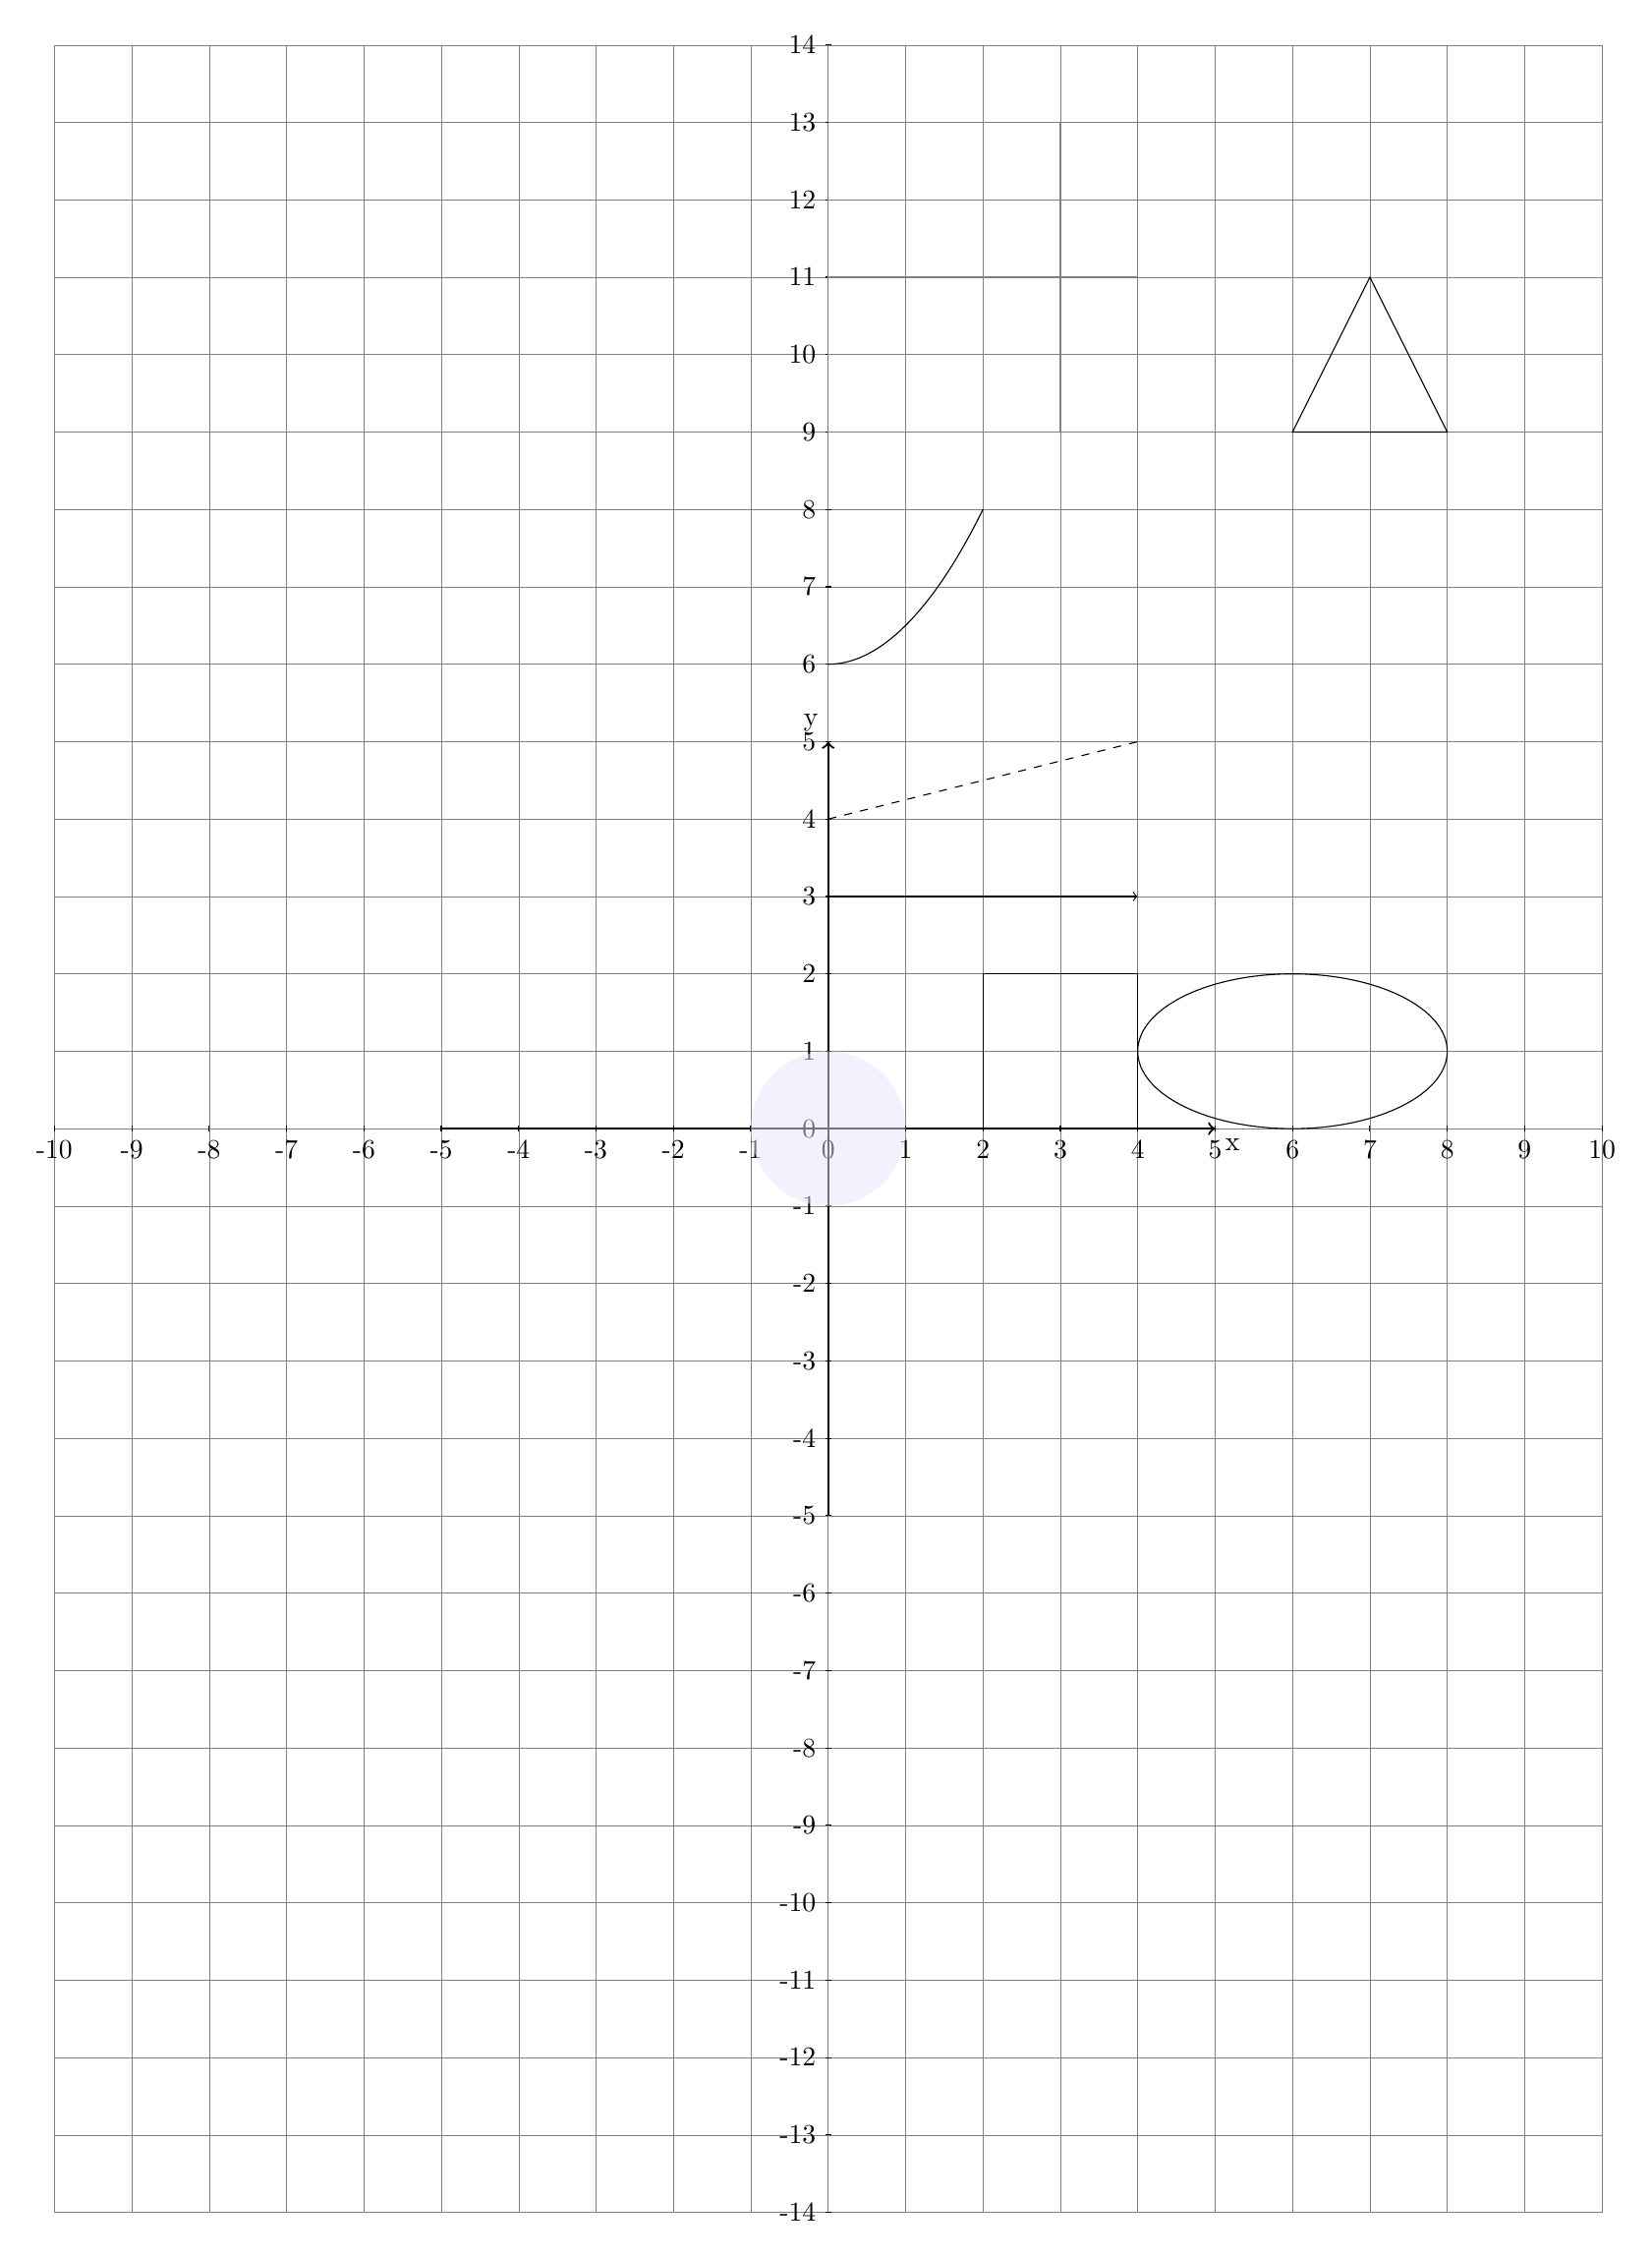
\begin{tikzpicture}[scale=1.0]
    % Draw the grid
    \draw[step=1cm,gray,very thin] (-10,-14) grid (10, 14);

    % Label x coordinates
    \foreach \x in {-10,-9,...,10}
        \draw (\x,1pt) -- (\x,-1pt) node[anchor=north] {\x};

    % Label y coordinates
    \foreach \y in {-14,-13,...,14}
        \draw (1pt,\y) -- (-1pt,\y) node[anchor=east] {\y};

    % Draw axes
    \draw[thick,->] (-5,0) -- (5,0) node[anchor=north west] {x};
    \draw[thick,->] (0,-5) -- (0,5) node[anchor=south east] {y};

    % Draw a blue filled circle
    \fill[blue!10, opacity=0.5] (0,0) circle (1cm);
    
    % Draw a rectangle
    \draw (2,0) rectangle (4,2);
    
    % Draw an ellipse
    \draw (6,1) ellipse (2cm and 1cm);
    
    % Draw a line with an arrowhead
    \draw[->] (0,3) -- (4,3);
    
    % Draw a dashed line
    \draw[dashed] (0,4) -- (4,5);
    
    % Draw a parabola
    \draw (0,6) parabola (2,8);
    
    % Draw a grid
    \draw[step=1cm,gray] (0,9) grid (4,13);
    
    % Draw a polygon
    \draw (6,9) -- (7,11) -- (8,9) -- cycle; 
\end{tikzpicture}
\end{document}

